\documentclass{beamer}
% \documentclass[handout]{beamer}
\usepackage{graphicx, color}
\usepackage{tikz}
\usepackage{subfigure}

% Use something like:
% % Use something like:
% % Use something like:
% \input{../../macros}

% groupings of objects.
\newcommand{\set}[1]{\left\{ #1 \right\}}
\newcommand{\seq}[1]{\left(#1\right)}
\newcommand{\ang}[1]{\langle#1\rangle}
\newcommand{\tuple}[1]{\left(#1\right)}

% numerical shortcuts.
\newcommand{\abs}[1]{\left| #1\right|}
\newcommand{\floor}[1]{\left\lfloor #1 \right\rfloor}
\newcommand{\ceil}[1]{\left\lceil #1 \right\rceil}

% linear algebra shortcuts.
\newcommand{\change}{\Delta}
\newcommand{\norm}[1]{\left\| #1\right\|}
\newcommand{\dprod}[1]{\langle#1\rangle}
\newcommand{\linspan}[1]{\langle#1\rangle}
\newcommand{\conj}[1]{\overline{#1}}
\newcommand{\gradient}{\nabla}
\newcommand{\der}{\frac{d}{dx}}
\newcommand{\lap}{\Delta}
\newcommand{\kron}{\otimes}
\newcommand{\nperp}{\nvdash}

\newcommand{\mat}[1]{\left( \begin{smallmatrix}#1 \end{smallmatrix} \right)}

% derivatives and limits
\newcommand{\partder}[2]{\frac{\partial #1}{\partial #2}}
\newcommand{\partdern}[3]{\frac{\partial^{#3} #1}{\partial #2^{#3}}}

% Arrows
\newcommand{\diverge}{\nearrow}
\newcommand{\notto}{\nrightarrow}
\newcommand{\up}{\uparrow}
\newcommand{\down}{\downarrow}
% gets and gives are defined!

% ordering operators
\newcommand{\oleq}{\preceq}
\newcommand{\ogeq}{\succeq}

% programming and logic operators
\newcommand{\dfn}{:=}
\newcommand{\assign}{:=}
\newcommand{\co}{\ co\ }
\newcommand{\en}{\ en\ }


% logic operators
\newcommand{\xor}{\oplus}
\newcommand{\Land}{\bigwedge}
\newcommand{\Lor}{\bigvee}
\newcommand{\finish}{$\Box$}
\newcommand{\contra}{\Rightarrow \Leftarrow}
\newcommand{\iseq}{\stackrel{_?}{=}}


% Set theory
\newcommand{\symdiff}{\Delta}
\newcommand{\union}{\cup}
\newcommand{\inters}{\cap}
\newcommand{\Union}{\bigcup}
\newcommand{\Inters}{\bigcap}
\newcommand{\nullSet}{\phi}

% graph theory
\newcommand{\nbd}{\Gamma}

% Script alphabets
% For reals, use \Re

% greek letters
\newcommand{\eps}{\epsilon}
\newcommand{\del}{\delta}
\newcommand{\ga}{\alpha}
\newcommand{\gb}{\beta}
\newcommand{\gd}{\del}
\newcommand{\gf}{\phi}
\newcommand{\gF}{\Phi}
\newcommand{\gl}{\lambda}
\newcommand{\gm}{\mu}
\newcommand{\gn}{\nu}
\newcommand{\gr}{\rho}
\newcommand{\gs}{\sigma}
\newcommand{\gt}{\theta}
\newcommand{\gx}{\xi}

\newcommand{\sw}{\sigma}
\newcommand{\SW}{\Sigma}
\newcommand{\ew}{\lambda}
\newcommand{\EW}{\Lambda}

\newcommand{\Del}{\Delta}
\newcommand{\gD}{\Delta}
\newcommand{\gG}{\Gamma}
\newcommand{\gO}{\Omega}
\newcommand{\gL}{\Lambda}
\newcommand{\gS}{\Sigma}

% Formatting shortcuts
\newcommand{\red}[1]{\textcolor{red}{#1}}
\newcommand{\blue}[1]{\textcolor{blue}{#1}}
\newcommand{\htext}[2]{\texorpdfstring{#1}{#2}}

% Statistics
\newcommand{\distr}{\sim}
\newcommand{\stddev}{\sigma}
\newcommand{\covmatrix}{\Sigma}
\newcommand{\mean}{\mu}
\newcommand{\param}{\gt}
\newcommand{\ftr}{\phi}

% General utility
\newcommand{\todo}[1]{\footnote{TODO: #1}}
\newcommand{\exclaim}[1]{{\textbf{\textit{#1}}}}
\newcommand{\tbc}{[\textbf{Incomplete}]}
\newcommand{\chk}{[\textbf{Check}]}
\newcommand{\oprob}{[\textbf{OP}]:}
\newcommand{\core}[1]{\textbf{Core Idea:}}
\newcommand{\why}{[\textbf{Find proof}]}
\newcommand{\opt}[1]{\textit{#1}}


\DeclareMathOperator*{\argmin}{arg\,min}
\DeclareMathOperator{\rank}{rank}
\newcommand{\redcol}[1]{\textcolor{red}{#1}}
\newcommand{\bluecol}[1]{\textcolor{blue}{#1}}
\newcommand{\greencol}[1]{\textcolor{green}{#1}}


\renewcommand{\~}{\htext{$\sim$}{~}}


% groupings of objects.
\newcommand{\set}[1]{\left\{ #1 \right\}}
\newcommand{\seq}[1]{\left(#1\right)}
\newcommand{\ang}[1]{\langle#1\rangle}
\newcommand{\tuple}[1]{\left(#1\right)}

% numerical shortcuts.
\newcommand{\abs}[1]{\left| #1\right|}
\newcommand{\floor}[1]{\left\lfloor #1 \right\rfloor}
\newcommand{\ceil}[1]{\left\lceil #1 \right\rceil}

% linear algebra shortcuts.
\newcommand{\change}{\Delta}
\newcommand{\norm}[1]{\left\| #1\right\|}
\newcommand{\dprod}[1]{\langle#1\rangle}
\newcommand{\linspan}[1]{\langle#1\rangle}
\newcommand{\conj}[1]{\overline{#1}}
\newcommand{\gradient}{\nabla}
\newcommand{\der}{\frac{d}{dx}}
\newcommand{\lap}{\Delta}
\newcommand{\kron}{\otimes}
\newcommand{\nperp}{\nvdash}

\newcommand{\mat}[1]{\left( \begin{smallmatrix}#1 \end{smallmatrix} \right)}

% derivatives and limits
\newcommand{\partder}[2]{\frac{\partial #1}{\partial #2}}
\newcommand{\partdern}[3]{\frac{\partial^{#3} #1}{\partial #2^{#3}}}

% Arrows
\newcommand{\diverge}{\nearrow}
\newcommand{\notto}{\nrightarrow}
\newcommand{\up}{\uparrow}
\newcommand{\down}{\downarrow}
% gets and gives are defined!

% ordering operators
\newcommand{\oleq}{\preceq}
\newcommand{\ogeq}{\succeq}

% programming and logic operators
\newcommand{\dfn}{:=}
\newcommand{\assign}{:=}
\newcommand{\co}{\ co\ }
\newcommand{\en}{\ en\ }


% logic operators
\newcommand{\xor}{\oplus}
\newcommand{\Land}{\bigwedge}
\newcommand{\Lor}{\bigvee}
\newcommand{\finish}{$\Box$}
\newcommand{\contra}{\Rightarrow \Leftarrow}
\newcommand{\iseq}{\stackrel{_?}{=}}


% Set theory
\newcommand{\symdiff}{\Delta}
\newcommand{\union}{\cup}
\newcommand{\inters}{\cap}
\newcommand{\Union}{\bigcup}
\newcommand{\Inters}{\bigcap}
\newcommand{\nullSet}{\phi}

% graph theory
\newcommand{\nbd}{\Gamma}

% Script alphabets
% For reals, use \Re

% greek letters
\newcommand{\eps}{\epsilon}
\newcommand{\del}{\delta}
\newcommand{\ga}{\alpha}
\newcommand{\gb}{\beta}
\newcommand{\gd}{\del}
\newcommand{\gf}{\phi}
\newcommand{\gF}{\Phi}
\newcommand{\gl}{\lambda}
\newcommand{\gm}{\mu}
\newcommand{\gn}{\nu}
\newcommand{\gr}{\rho}
\newcommand{\gs}{\sigma}
\newcommand{\gt}{\theta}
\newcommand{\gx}{\xi}

\newcommand{\sw}{\sigma}
\newcommand{\SW}{\Sigma}
\newcommand{\ew}{\lambda}
\newcommand{\EW}{\Lambda}

\newcommand{\Del}{\Delta}
\newcommand{\gD}{\Delta}
\newcommand{\gG}{\Gamma}
\newcommand{\gO}{\Omega}
\newcommand{\gL}{\Lambda}
\newcommand{\gS}{\Sigma}

% Formatting shortcuts
\newcommand{\red}[1]{\textcolor{red}{#1}}
\newcommand{\blue}[1]{\textcolor{blue}{#1}}
\newcommand{\htext}[2]{\texorpdfstring{#1}{#2}}

% Statistics
\newcommand{\distr}{\sim}
\newcommand{\stddev}{\sigma}
\newcommand{\covmatrix}{\Sigma}
\newcommand{\mean}{\mu}
\newcommand{\param}{\gt}
\newcommand{\ftr}{\phi}

% General utility
\newcommand{\todo}[1]{\footnote{TODO: #1}}
\newcommand{\exclaim}[1]{{\textbf{\textit{#1}}}}
\newcommand{\tbc}{[\textbf{Incomplete}]}
\newcommand{\chk}{[\textbf{Check}]}
\newcommand{\oprob}{[\textbf{OP}]:}
\newcommand{\core}[1]{\textbf{Core Idea:}}
\newcommand{\why}{[\textbf{Find proof}]}
\newcommand{\opt}[1]{\textit{#1}}


\DeclareMathOperator*{\argmin}{arg\,min}
\DeclareMathOperator{\rank}{rank}
\newcommand{\redcol}[1]{\textcolor{red}{#1}}
\newcommand{\bluecol}[1]{\textcolor{blue}{#1}}
\newcommand{\greencol}[1]{\textcolor{green}{#1}}


\renewcommand{\~}{\htext{$\sim$}{~}}


% groupings of objects.
\newcommand{\set}[1]{\left\{ #1 \right\}}
\newcommand{\seq}[1]{\left(#1\right)}
\newcommand{\ang}[1]{\langle#1\rangle}
\newcommand{\tuple}[1]{\left(#1\right)}

% numerical shortcuts.
\newcommand{\abs}[1]{\left| #1\right|}
\newcommand{\floor}[1]{\left\lfloor #1 \right\rfloor}
\newcommand{\ceil}[1]{\left\lceil #1 \right\rceil}

% linear algebra shortcuts.
\newcommand{\change}{\Delta}
\newcommand{\norm}[1]{\left\| #1\right\|}
\newcommand{\dprod}[1]{\langle#1\rangle}
\newcommand{\linspan}[1]{\langle#1\rangle}
\newcommand{\conj}[1]{\overline{#1}}
\newcommand{\gradient}{\nabla}
\newcommand{\der}{\frac{d}{dx}}
\newcommand{\lap}{\Delta}
\newcommand{\kron}{\otimes}
\newcommand{\nperp}{\nvdash}

\newcommand{\mat}[1]{\left( \begin{smallmatrix}#1 \end{smallmatrix} \right)}

% derivatives and limits
\newcommand{\partder}[2]{\frac{\partial #1}{\partial #2}}
\newcommand{\partdern}[3]{\frac{\partial^{#3} #1}{\partial #2^{#3}}}

% Arrows
\newcommand{\diverge}{\nearrow}
\newcommand{\notto}{\nrightarrow}
\newcommand{\up}{\uparrow}
\newcommand{\down}{\downarrow}
% gets and gives are defined!

% ordering operators
\newcommand{\oleq}{\preceq}
\newcommand{\ogeq}{\succeq}

% programming and logic operators
\newcommand{\dfn}{:=}
\newcommand{\assign}{:=}
\newcommand{\co}{\ co\ }
\newcommand{\en}{\ en\ }


% logic operators
\newcommand{\xor}{\oplus}
\newcommand{\Land}{\bigwedge}
\newcommand{\Lor}{\bigvee}
\newcommand{\finish}{$\Box$}
\newcommand{\contra}{\Rightarrow \Leftarrow}
\newcommand{\iseq}{\stackrel{_?}{=}}


% Set theory
\newcommand{\symdiff}{\Delta}
\newcommand{\union}{\cup}
\newcommand{\inters}{\cap}
\newcommand{\Union}{\bigcup}
\newcommand{\Inters}{\bigcap}
\newcommand{\nullSet}{\phi}

% graph theory
\newcommand{\nbd}{\Gamma}

% Script alphabets
% For reals, use \Re

% greek letters
\newcommand{\eps}{\epsilon}
\newcommand{\del}{\delta}
\newcommand{\ga}{\alpha}
\newcommand{\gb}{\beta}
\newcommand{\gd}{\del}
\newcommand{\gf}{\phi}
\newcommand{\gF}{\Phi}
\newcommand{\gl}{\lambda}
\newcommand{\gm}{\mu}
\newcommand{\gn}{\nu}
\newcommand{\gr}{\rho}
\newcommand{\gs}{\sigma}
\newcommand{\gt}{\theta}
\newcommand{\gx}{\xi}

\newcommand{\sw}{\sigma}
\newcommand{\SW}{\Sigma}
\newcommand{\ew}{\lambda}
\newcommand{\EW}{\Lambda}

\newcommand{\Del}{\Delta}
\newcommand{\gD}{\Delta}
\newcommand{\gG}{\Gamma}
\newcommand{\gO}{\Omega}
\newcommand{\gL}{\Lambda}
\newcommand{\gS}{\Sigma}

% Formatting shortcuts
\newcommand{\red}[1]{\textcolor{red}{#1}}
\newcommand{\blue}[1]{\textcolor{blue}{#1}}
\newcommand{\htext}[2]{\texorpdfstring{#1}{#2}}

% Statistics
\newcommand{\distr}{\sim}
\newcommand{\stddev}{\sigma}
\newcommand{\covmatrix}{\Sigma}
\newcommand{\mean}{\mu}
\newcommand{\param}{\gt}
\newcommand{\ftr}{\phi}

% General utility
\newcommand{\todo}[1]{\footnote{TODO: #1}}
\newcommand{\exclaim}[1]{{\textbf{\textit{#1}}}}
\newcommand{\tbc}{[\textbf{Incomplete}]}
\newcommand{\chk}{[\textbf{Check}]}
\newcommand{\oprob}{[\textbf{OP}]:}
\newcommand{\core}[1]{\textbf{Core Idea:}}
\newcommand{\why}{[\textbf{Find proof}]}
\newcommand{\opt}[1]{\textit{#1}}


\DeclareMathOperator*{\argmin}{arg\,min}
\DeclareMathOperator{\rank}{rank}
\newcommand{\redcol}[1]{\textcolor{red}{#1}}
\newcommand{\bluecol}[1]{\textcolor{blue}{#1}}
\newcommand{\greencol}[1]{\textcolor{green}{#1}}


\renewcommand{\~}{\htext{$\sim$}{~}}

% Use something like:
% % Use something like:
% % Use something like:
% \input{../../presentationMacros}

% Useful shorthands.
\newcommand{\pitem}{\pause \item}
\AtBeginSection[]
{
   \begin{frame}
       \frametitle{Outline}
       \tableofcontents[currentsection]
   \end{frame}
}

\AtBeginSubsection[]
{
   \begin{frame}
       \frametitle{Outline}
       \tableofcontents[currentsection,currentsubsection]
   \end{frame}
}

\AtBeginSubsubsection[]
{
   \begin{frame}
       \frametitle{Outline}
       \tableofcontents[currentsection,currentsubsection, currentsubsubsection]
   \end{frame}
}


% Useful shorthands.
\newcommand{\pitem}{\pause \item}
\AtBeginSection[]
{
   \begin{frame}
       \frametitle{Outline}
       \tableofcontents[currentsection]
   \end{frame}
}

\AtBeginSubsection[]
{
   \begin{frame}
       \frametitle{Outline}
       \tableofcontents[currentsection,currentsubsection]
   \end{frame}
}

\AtBeginSubsubsection[]
{
   \begin{frame}
       \frametitle{Outline}
       \tableofcontents[currentsection,currentsubsection, currentsubsubsection]
   \end{frame}
}


% Useful shorthands.
\newcommand{\pitem}{\pause \item}
\AtBeginSection[]
{
   \begin{frame}
       \frametitle{Outline}
       \tableofcontents[currentsection]
   \end{frame}
}

\AtBeginSubsection[]
{
   \begin{frame}
       \frametitle{Outline}
       \tableofcontents[currentsection,currentsubsection]
   \end{frame}
}

\AtBeginSubsubsection[]
{
   \begin{frame}
       \frametitle{Outline}
       \tableofcontents[currentsection,currentsubsection, currentsubsubsection]
   \end{frame}
}


\usetheme{Warsaw}
\pgfdeclarelayer{background}
\pgfsetlayers{background,main}

\title{Affiliation Recommendation using Auxiliary Social Networks}
% \author{Vishvas Vasuki, Nagarajan Natarajan, Zhengdong Lu, Inderjit Dhillon}
% \date{\today}

\begin{document}

% \AtBeginSection[]
% {
%    \begin{frame}
%        \frametitle{Outline}
%        \tableofcontents[currentsection]
%    \end{frame}
% }

% \AtBeginSubsection[]
% {
%    \begin{frame}
%        \frametitle{Outline}
%        \tableofcontents[currentsection,currentsubsection]
%    \end{frame}
% }
% 
% \bAtBeginSubsubsection[]
% {
%    \begin{frame}
%        \frametitle{Outline}
%        \tableofcontents[currentsection,currentsubsection, currentsubsubsection]
%    \end{frame}
% }

\frame{\titlepage}
\section{Outline}
\begin{frame}
\frametitle{What to look out for?}
\begin{itemize}
\pitem Affiliation recommendation problem.
\pitem Affiliation recommendation algorithms.
\end{itemize}
\end{frame}

\section{Social network analysis}
\subsection{Social and affiliation networks}
\begin{frame}
\frametitle{Social networks}
\begin{itemize}
\pitem \todo{Pictures of orkut, facebook, yeast network.}
\pitem Not necessarily among people - Yeast gene network.
\end{itemize}
\end{frame}

\begin{frame}
\frametitle{Social network S: An undirected graph.}

\tikzstyle{vertex}=[circle, fill=magenta!25,minimum size=15pt,inner sep=0pt]
\tikzstyle{edge} = [draw,thick,-]

\begin{center}
\begin{tikzpicture}[scale=2]
    % Social network
    \foreach \pos/\name/\user/\anchor in {{(0,1)/4/Dave/left}, {(0,2)/3/Carol/left}, {(1,1)/2/Bob/right},{(1,2)/1/Alice/right},{(1,3)/5/Eve/above}}
        \node[vertex] (u\name) [label=\anchor:\user] at \pos {$\name$};
    \foreach \source/ \dest in {u1/u2, u1/u3, u1/u4, u2/u4, u1/u5}
        \path[edge] (\source) -- (\dest);

    \draw (0.5,3.5) node[above]{$\mathcal{S}$};
\end{tikzpicture}
\end{center}
\end{frame}

\begin{frame}
\frametitle{Affiliation networks}
\begin{itemize}
\pitem Pictures of orkut and facebook communities.
\pitem Not necessarily among people - gene-disease network.
\end{itemize}
\end{frame}

\begin{frame}
\frametitle{Affiliation network A: A bipartite graph.}
\tikzstyle{user}=[circle, fill=magenta!25,minimum size=15pt,inner sep=0pt]
\tikzstyle{community}=[circle, fill=cyan!25,minimum size=15pt,inner sep=0pt]
\tikzstyle{edge} = [draw,thick,-]
\begin{center}
\begin{tikzpicture}[scale=1]
    % First we draw the vertices
    \foreach \pos/\name/\user in {{(0,0)/5/Eve}, {(0,1)/4/Dave}, {(0,2)/3/Carol}, {(0,3)/2/Bob},{(0,4)/1/Alice}}
        \node[user] (u\name) [label=left:\user] at \pos {$\name$};
    \foreach \pos/\name/\group in {{(2,0)/6/Tennis}, {(2,1)/5/Math}, {(2,2)/4/Soccer},{(2,3)/3/Science}, {(2,4)/2/Jazz},{(2,5)/1/Salsa},{(2,-1)/7/Cryptography}}
        \node[community] (c\name)  [label=right:\group] at \pos {$\name$};
    
    % Connect vertices with edges
    \foreach \source/ \dest in {u1/c1,u1/c4,u2/c1,u3/c5,u3/c6,u4/c2,u1/c7,u2/c7,u3/c7,u4/c7,u5/c3}
        \path[edge] (\source) -- (\dest);
        
    \draw (1,5) node[above]{$\mathcal{A}$}; 
\end{tikzpicture}
\end{center}
\end{frame}

\subsection{Social network analysis: Problems}
\begin{frame}
\frametitle{Problems in social network analysis.}
\begin{itemize}
\pitem Modelling network evolution.
\pitem Link prediction.
\pitem Community identification.
\end{itemize}
\end{frame}

\begin{frame}
\frametitle{Affiliation Recommendation.}
\begin{itemize}
\pitem Exploiting social network in making affiliation recommendations.
\pitem Generalizable to the item recommendation problem.
\begin{figure}
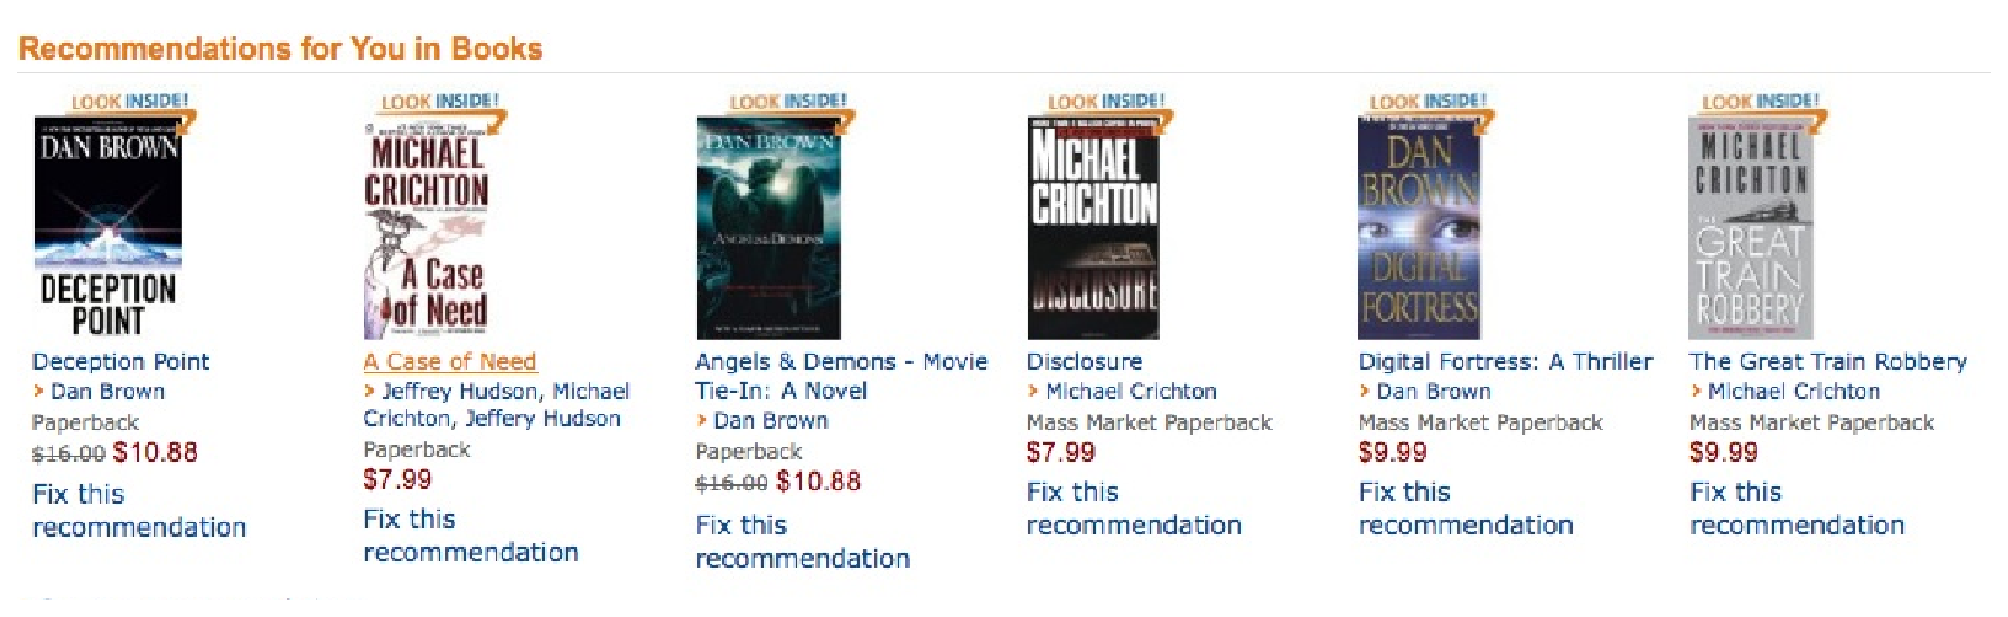
\includegraphics[scale=0.25]{figures/amazonRecommendations.eps}
\end{figure}
\end{itemize}
\end{frame}

\section{Recommendation algorithms}
\subsection{Modelling user-affiliation affinity}
\begin{frame}
\frametitle{The combined network}
\begin{itemize}
 \pitem $\gl$: relative weight associated with information in $S$.
 \pitem $\bD$: unobserved.
\end{itemize}
\tikzstyle{user}=[circle, fill=magenta!25,minimum size=15pt,inner sep=0pt]
\tikzstyle{community}=[circle, fill=cyan!25,minimum size=15pt,inner sep=0pt]
\tikzstyle{userUserEdge} = [draw,thick,-, color=red]
\tikzstyle{userGroupEdge} = [draw,thick,-, color=blue]
\begin{tikzpicture}[scale=0.8]
    % Combined network
    \foreach \pos/\name/\user in {{(5,0)/5/Eve}, {(5,1)/4/Dave}, {(5,2)/3/Carol}, {(5,3)/2/Bob},{(5,4)/1/Alice}}
        \node[user] (u\name) [label=left:\user] at \pos {$\name$};
    \foreach \pos/\name/\group in {{(7,0)/6/Tennis}, {(7,1)/5/Math}, {(7,2)/4/Soccer},{(7,3)/3/Science}, {(7,4)/2/Jazz},{(7,5)/1/Salsa},{(7,-1)/7/Cryptography}}
        \node[community] (c\name)  [label=right:\group] at \pos {$\name$};
    \foreach \source/ \dest in {u1/u2, u1/u3, u1/u4, u2/u4,u1/u5}
       \path (\source) edge [color=red, bend right] (\dest);
    \foreach \source/ \dest in {u1/c1,u1/c4,u2/c1,u3/c5,u3/c6,u4/c2,u1/c7,u2/c7,u3/c7,u4/c7,u5/c3}
        \path[userGroupEdge] (\source) -- (\dest);

    \draw (5,5) node[above]{\large{$\mathcal{C}$}};
    
    % Write the combined adjacency matrix
    \draw (0,2) node[above] {\large{$\bC(\gl, \bD) = \begin{bmatrix} \gl \red{S}& \blue{A}\\ \blue{A^{T}}& \bD\end{bmatrix}$}};
\end{tikzpicture}
\end{frame}

\subsection{Latent factors model}
\begin{frame}
\frametitle{Modelling A alone}
\begin{itemize}
\pitem User-group affinity as a product of low dimensional vectors: $\bA_{i, j} \approx \dprod{\bU(i, :), \bG(i, :)}$.
\pitem $\bA \approx \bU \bG, rank(\bU) \leq k, rank(\bG) \leq k$. (U as user preferences, G as group properties.)
\pitem For user $j$, recommend affiliations with high affinity.
\end{itemize}
\end{frame}

\begin{frame}
\frametitle{Modelling C}
\begin{itemize}
\pitem A \textbf{good model} will account for edges in $\bS$ too. $\bC(\gl, \bD) \approx \mat{\bV_1\\ \bV_2}\bL \mat{\bV_1^{T} \bV_2^{T}}$, rank of $\bV_i$ and $\bL$ $\leq k$.
\pitem So $\bA \approx \bV_1 \bL \bV_2^T$.
\pitem $\bV_1 \bL \bV_2^T$ is a similarity score matrix for ranking potential affiliations.
\end{itemize}
\end{frame}


\subsection{Graph proximity model}
\begin{frame}
\frametitle{Proximity between users in a social network}
$\bC^{2}_{i,j}$ : Number of paths of length 2 between $i$ and $j$.

\tikzstyle{vertex}=[circle, fill=magenta!25,minimum size=15pt,inner sep=0pt]
\tikzstyle{selected vertex}=[vertex, fill=red]
\tikzstyle{unselect vertex}=[vertex, fill=magenta!25]
\tikzstyle{edge} = [draw,thick,-]
\tikzstyle{selected edge} = [edge,line width=3pt,red!25]
\tikzstyle{unselect edge} = [selected edge, red]

\begin{center}
\begin{tikzpicture}[scale=2]
    % Social network
    \node[vertex] (u4) at (0,1) {};
    \node[vertex] (u3) at (0,2) {$i$};
    \node[vertex] (u2) at (1,1) {$j$};
    \node[vertex] (u1) at (1,2) {};
    \node[vertex] (u5) at (1,3) {};
    
    \foreach \source/ \dest in {u1/u2, u1/u3, u1/u4, u2/u4, u1/u5}
        \path[edge] (\source) -- (\dest);

    \draw (0.5,3.5) node[above]{$\mathcal{C} \to \mathcal{C}^{2}$};
    \begin{pgfonlayer}{background}
        \pause
        \foreach \source / \dest in {3/1, 1/2}
            \path<+->[selected edge] (u\source) -- (u\dest);
        \foreach \source / \dest / \fr in {3/1/4,1/2/4}
            \path<\fr->[unselect edge] (u\source) -- (u\dest);
    \end{pgfonlayer}
\end{tikzpicture}
\end{center}
\end{frame}

\begin{frame}
\frametitle{Proximity between users in a social network}
$\bC^{3}_{i,j}$ : Number of paths of length 3 between $i$ and $j$.

\tikzstyle{vertex}=[circle, fill=magenta!25,minimum size=15pt,inner sep=0pt]
\tikzstyle{selected vertex}=[vertex, fill=red]
\tikzstyle{unselect vertex}=[vertex, fill=magenta!25]
\tikzstyle{edge} = [draw,thick,-]
\tikzstyle{selected edge} = [edge,line width=3pt,red!25]
\tikzstyle{unselect edge} = [selected edge, red]

\begin{center}
\begin{tikzpicture}[scale=2]
    % Social network
    \node[vertex] (u4) at (0,1) {};
    \node[vertex] (u3) at (0,2) {$i$};
    \node[vertex] (u2) at (1,1) {$j$};
    \node[vertex] (u1) at (1,2) {};
    \node[vertex] (u5) at (1,3) {};
    \foreach \source/ \dest in {u1/u2, u1/u3, u1/u4, u2/u4, u1/u5}
        \path[edge] (\source) -- (\dest);

    \draw (0.5,3.5) node[above]{$\mathcal{C} \to \mathcal{C}^{3}$};;
    \begin{pgfonlayer}{background}
        \pause
        \foreach \source / \dest in {3/1,1/4, 4/2}
            \path<+->[selected edge] (u\source) -- (u\dest);
        \foreach \source / \dest / \fr in {3/1/5,1/4/5,4/2/5}
            \path<\fr->[unselect edge] (u\source) -- (u\dest);
    \end{pgfonlayer}
\end{tikzpicture}
\end{center}
\end{frame}

\begin{frame}
\frametitle{Graph proximity Model}
\begin{itemize}
\pitem $\text{Proximity}(i, j) = \gb^{2} \bC^{2}_{i,j} + \gb^{3}\bC^3_{i,j} + \dots$
\pitem Known as Katz measure, when the series is convergent ($\|\gb C \|_{2} < 1$).
\pitem To save time, compute the truncated Katz measure, $\textsf{tKatz}(\bC, \gb, k) = \sum_{i=1}^{k} \gb^i \bC^i$.
\pitem Recommend user-group affiliations based on proximity in $\bC$.
\end{itemize}
\end{frame}

\begin{frame}
\frametitle{User-group proximity: Paths considered}
\begin{itemize}
\pitem $
\text{user $i$ } \, \xrightarrow{\bS}\, \text{user $j$ } \,\xrightarrow{\bA} \, \text{ group $n$ (in $\bC^2$)}$

\pitem $
\text{user $i$ } \, \xrightarrow{\bS} \, \text{user $j$ } \, \xrightarrow{\bA\bA^T} \, \text{ $k$ }\, \xrightarrow{\bA}\, \text{ group $n$ (in $\bC^4$)}$
\end{itemize}
\end{frame}


\subsection{Scalability for graph proximity model}
\begin{frame}
\frametitle{Scalable recommenders for the graph proximity model}
\begin{itemize}
\pitem $\textsf{tKatz}(\bC, \gb, k) = \sum_{i=1}^{k} \gb^i \bC^i $.
\pitem $\bC^i$ gets denser, so hard to compute.
\pitem Use Low rank approximations of $\bC \approx \bV\Lambda^{i}\bV^{T}$.  Use $\bC^i \approx \bV\Lambda^{i}\bV^{T}$. \cite{vasukiScalableAffiliationRec}
\end{itemize}
\end{frame}

\begin{frame}
\frametitle{Common Subspace Approximation}
\begin{itemize}
\pitem $\textsf{tKatz}(\bC;\gb,3)_{12} = \gb \bA + \gb^2 \lambda \bS \bA +  \gb^3(\lambda^2 \bS^2 \bA + \bA \bA^T \bA)$.
\pitem $(\bA\bA^{T})^i, \bS^{i}, (\bA\bA^{T})^{j}\bS^{i}$ gets denser, so hard to compute.
\pitem Use $\bS \approx \bQ (\bQ^T \bS \bQ) \bQ^T \equiv\bQ \bD_\bS \bQ^T,  \bA \approx \bQ (\bQ^T \bA\bV) \bV^T \equiv\bQ \bD_\bA \bV^T$.
\pitem Now $(\bA\bA^{T})^i \approx \bQ(\bD_\bA\bD_\bA^{T})^{i} \bQ^T$, $(\bS)^i \approx \bQ\bD_\bS^{i} \bQ^T$, $(\bS\bA\bA^{T}) \approx \bQ\bD_\bS (\bD_\bA\bD_\bA^{T}) \bQ^T$.
\end{itemize}
\end{frame}

\section{Experiments}
\subsection{Datasets and their statistics}
\begin{frame}
\frametitle{Data sets}
\begin{figure}
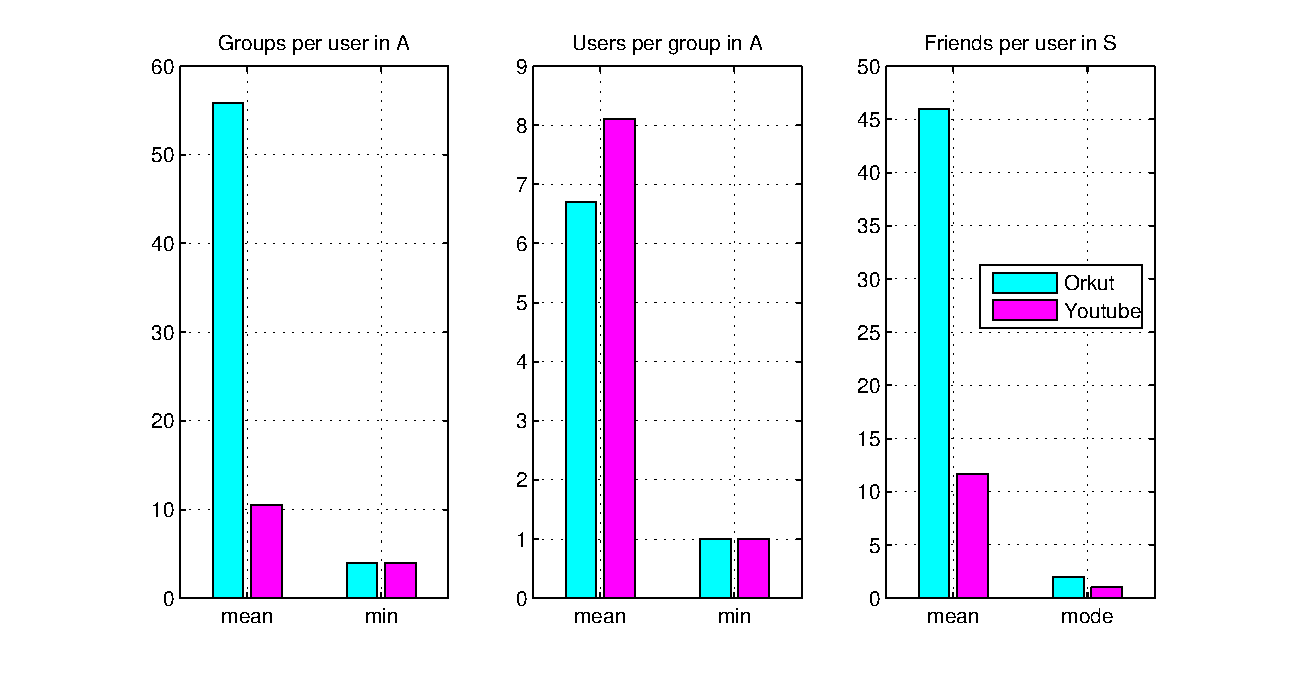
\includegraphics[scale=0.4]{figures/stats.eps}
\caption{Statistics of extracted social and affiliation networks: \emph{Orkut} and \emph{Youtube} data sets \cite{Mislove}; Orkut: \blue{$N_{u} = 9123, N_{g} = 75546$}. Youtube: \blue{$N_{u} =16575, N_{g} = 21326$}.}
\end{figure}
\end{frame}

\subsection{Evaluation methods}
\begin{frame}
\frametitle{Evaluation methods}
\begin{itemize}
\pitem Choosing appropriate evaluation method --- Not obvious!
\pitem ``Global'' sensitivity vs ``Per-user'' sensitivity.
\pause
\begin{figure}[h]
  \begin{center}
    \subfigure[Orkut dataset]{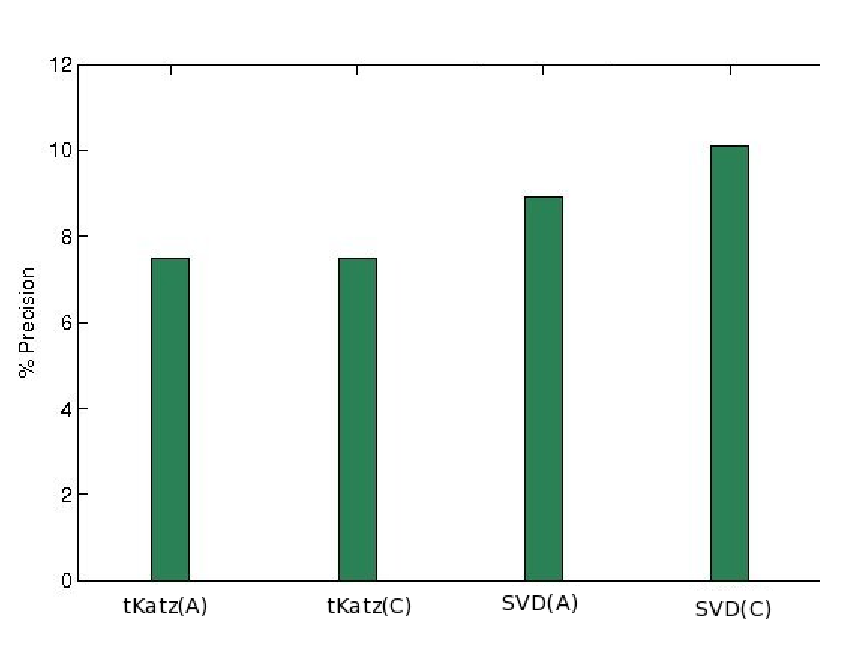
\includegraphics[scale=0.25]{../paper/OrkutLinkPredictionEvaluation.eps}}
    \subfigure[Youtube dataset]{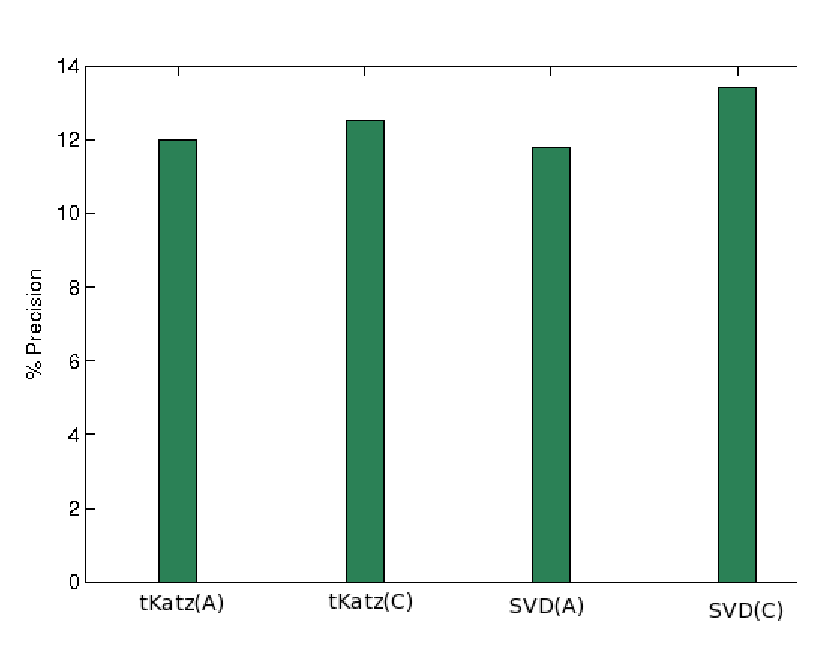
\includegraphics[scale=0.25]{../paper/YoutubeLinkPredictionEvaluation.eps}}
  \end{center}
  \caption{Comparison of recommendation algorithms using ``global sensitivity''.}
\end{figure}
\pitem Consider the top 50 recommendations made for a user.
\end{itemize}
\end{frame}

\subsection{Results and discussion}
\begin{frame}
\frametitle{Results}
\begin{figure}[h]
  \begin{center}
    \subfigure[Orkut dataset]{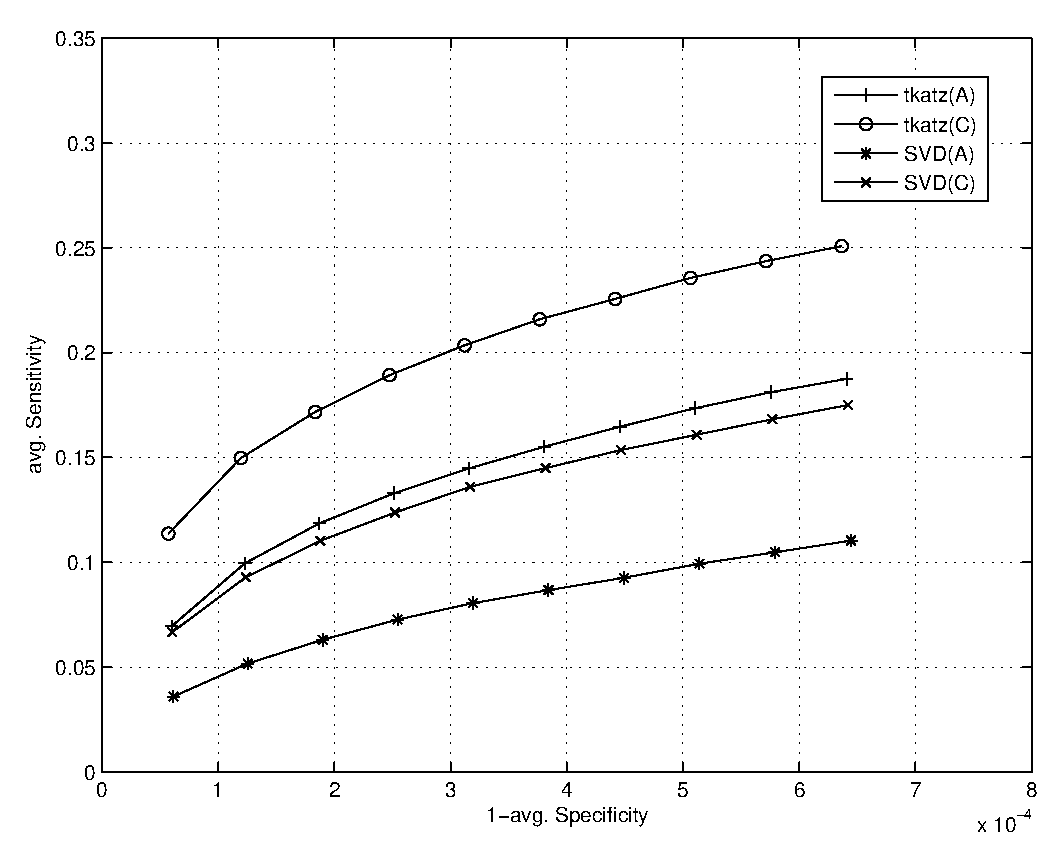
\includegraphics[scale=0.25]{../paper/summaryOrkut.eps}}
    \subfigure[Youtube dataset]{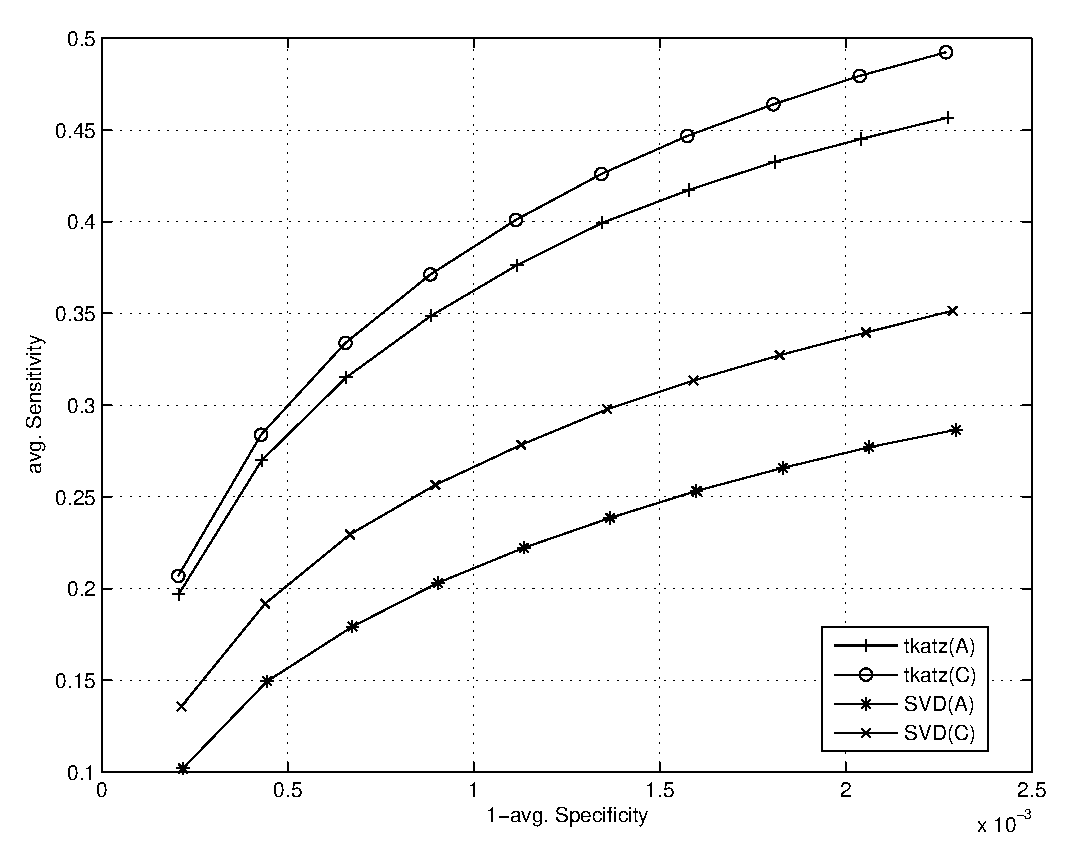
\includegraphics[scale=0.25]{../paper/summaryYoutube.eps}}
  \end{center}
  \caption{Comparison of recommendation algorithms using ``Per-user'' sensitivity.}
\end{figure}
\end{frame}

\begin{frame}
\frametitle{Results}
\begin{figure}[h]
  \begin{center}
    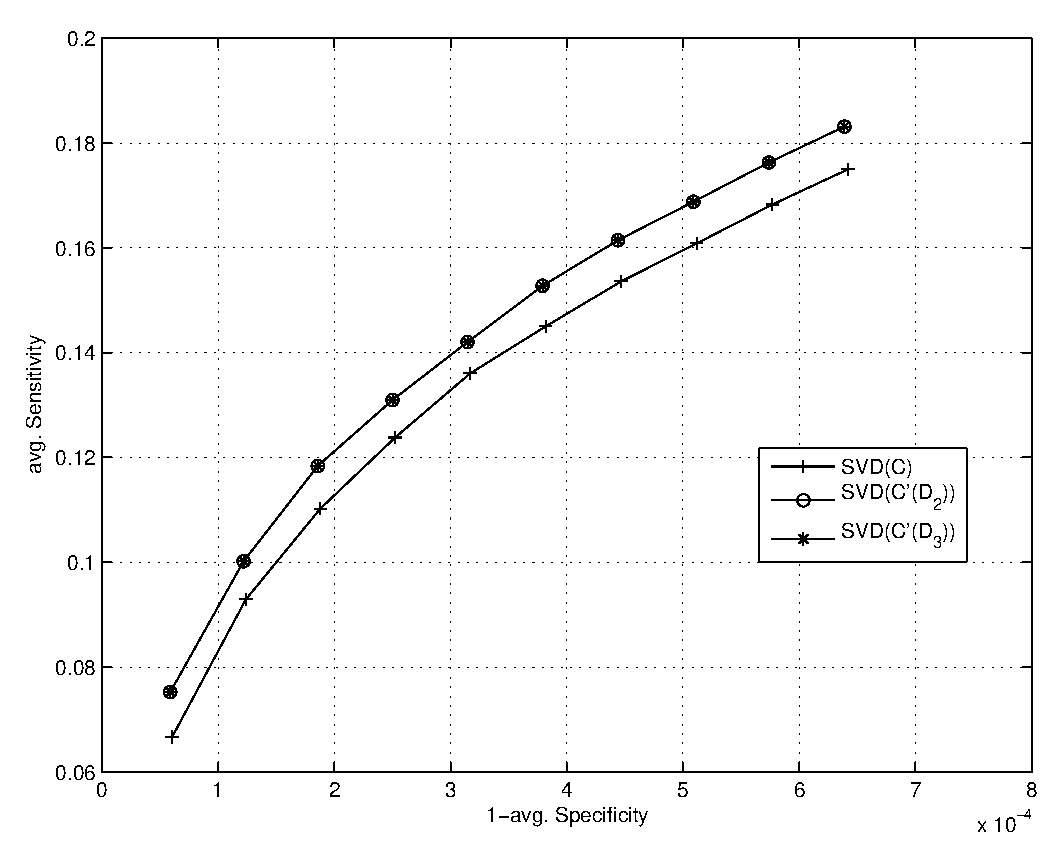
\includegraphics[scale=0.3]{../paper/summarySVDOrkut.eps}
  \end{center}
  \caption{Comparison of latent factors based algorithms for various choices of $\bD$, for the Orkut dataset: $\bD_{2} = \bA^{T}\bA, \bD_{3} = \lambda \bA^{T}\bA$.}
\end{figure}
\begin{itemize}
\pitem Choice of $\bD$ is immaterial! (Consistent on Youtube).
\end{itemize}
\end{frame}

\begin{frame}
\frametitle{Results}
\begin{figure}
  \begin{center}
    \subfigure[Orkut-1c data set]{\includegraphics[scale=0.25]{../journalPaper/summarySVDKatzOrkut.eps}}
    \subfigure[Youtube-1c data set]{\includegraphics[scale=0.25]{../journalPaper/summarySVDKatzYoutube.eps}}
  \end{center}
  \caption{Scalable approximations}
\end{figure}
\end{frame}

\begin{frame}
\frametitle{Results}
\begin{figure}
  \begin{center}
    \subfigure[Orkut-1c data set]{\includegraphics[scale=0.25]{../journalPaper/summaryScalabilityOrkut.eps}}
    \subfigure[Youtube-1c data set]{\includegraphics[scale=0.25]{../journalPaper/summaryScalabilityYoutube.eps}}
  \end{center}
  \caption{Scalable approximations: Clustering}
\end{figure}
\end{frame}

\begin{frame}
\frametitle{Results}
\begin{figure}
  \begin{center}
    \subfigure[Effect of changing the number of clusters.]{\includegraphics[scale=0.25]{../journalPaper/summaryClusteredMethodsClusterDependencyYoutube.eps}}
    \subfigure[Effect of changing the number of factors.]{\includegraphics[scale=0.25]{../journalPaper/summaryRankDependencyYoutube.eps}}
  \end{center}
\end{figure}
\end{frame}

\section{Conclusion}
\begin{frame}
\frametitle{Conclusion}
\begin{itemize}
\pitem Friendship network is indeed useful in recommending affiliations!
\pitem Community recommendation -- link prediction perspective.
\pitem Two ways of modeling the information from auxiliary networks.
\pitem Choice of evaluation strategy is important.
\end{itemize}
\end{frame}

\begin{frame}
\frametitle{Future work}
\begin{itemize}
\pitem Using affiliation networks for link prediction in friendship networks -- Seems harder.
\pitem More sources of information -- How do you use them all?
\pitem Huge networks -- Scalability.
\end{itemize}
\end{frame}

\begin{frame}
\frametitle{The take home message}
\begin{itemize}
\pitem Graph proximity on Combined user/ item network $\to$ Good item recommendations.
\pitem Can make this scalable.
\end{itemize}
\end{frame}

\begin{frame}
\frametitle{References}
% 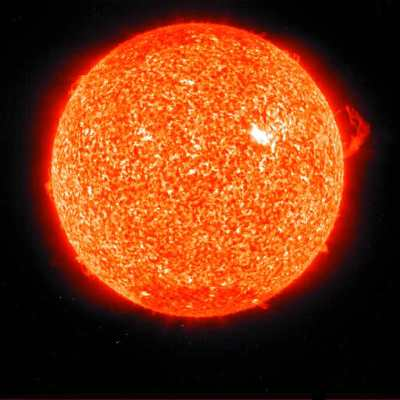
\includegraphics[scale=.5]{images/sun.jpg}
\nocite{vasukiNatarajan, vasukiScalableAffiliationRec}
\end{frame}

\bibliographystyle{plain}
\bibliography{../paper/references}


\end{document}
